\ifx \allfiles \undefined
\documentclass{article}
  \usepackage{ctex, graphicx, float}
  \begin{document}
\fi

  \section{CompoNet结构说明}
  \subsection{功能}
    接受一段音符序列,对其进行“续写”。
  \subsection{输入}
    我们在已有的mid文件中随机选取了一些统计了音符的四个
    要素(pitch,dynamic,rhythmValue,duration)的分布情况如下图所示:
    
    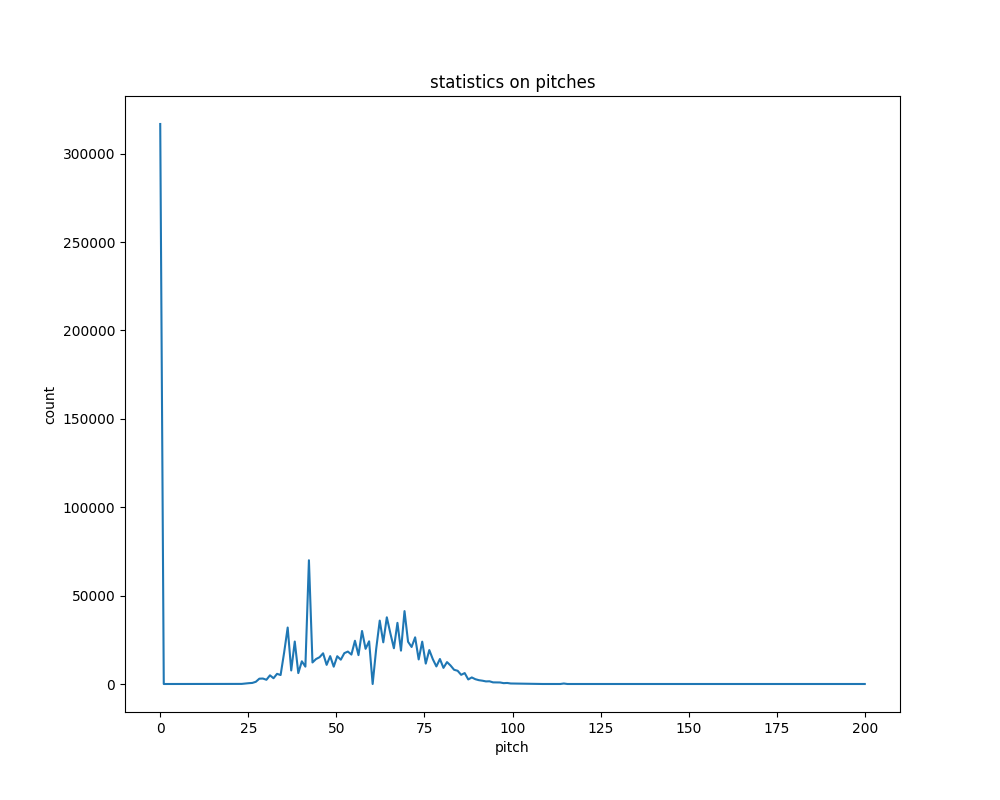
\includegraphics[width=.9\textwidth]{picture/pitches.png}
      
    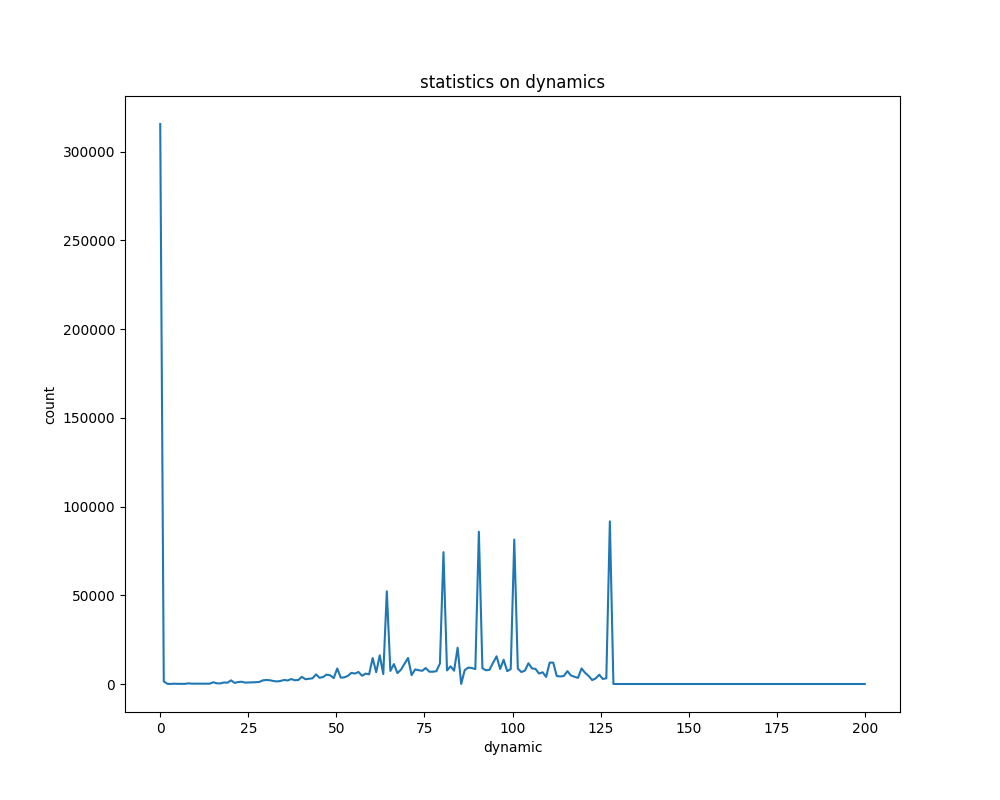
\includegraphics[width=.9\textwidth]{picture/dynamics.png}

    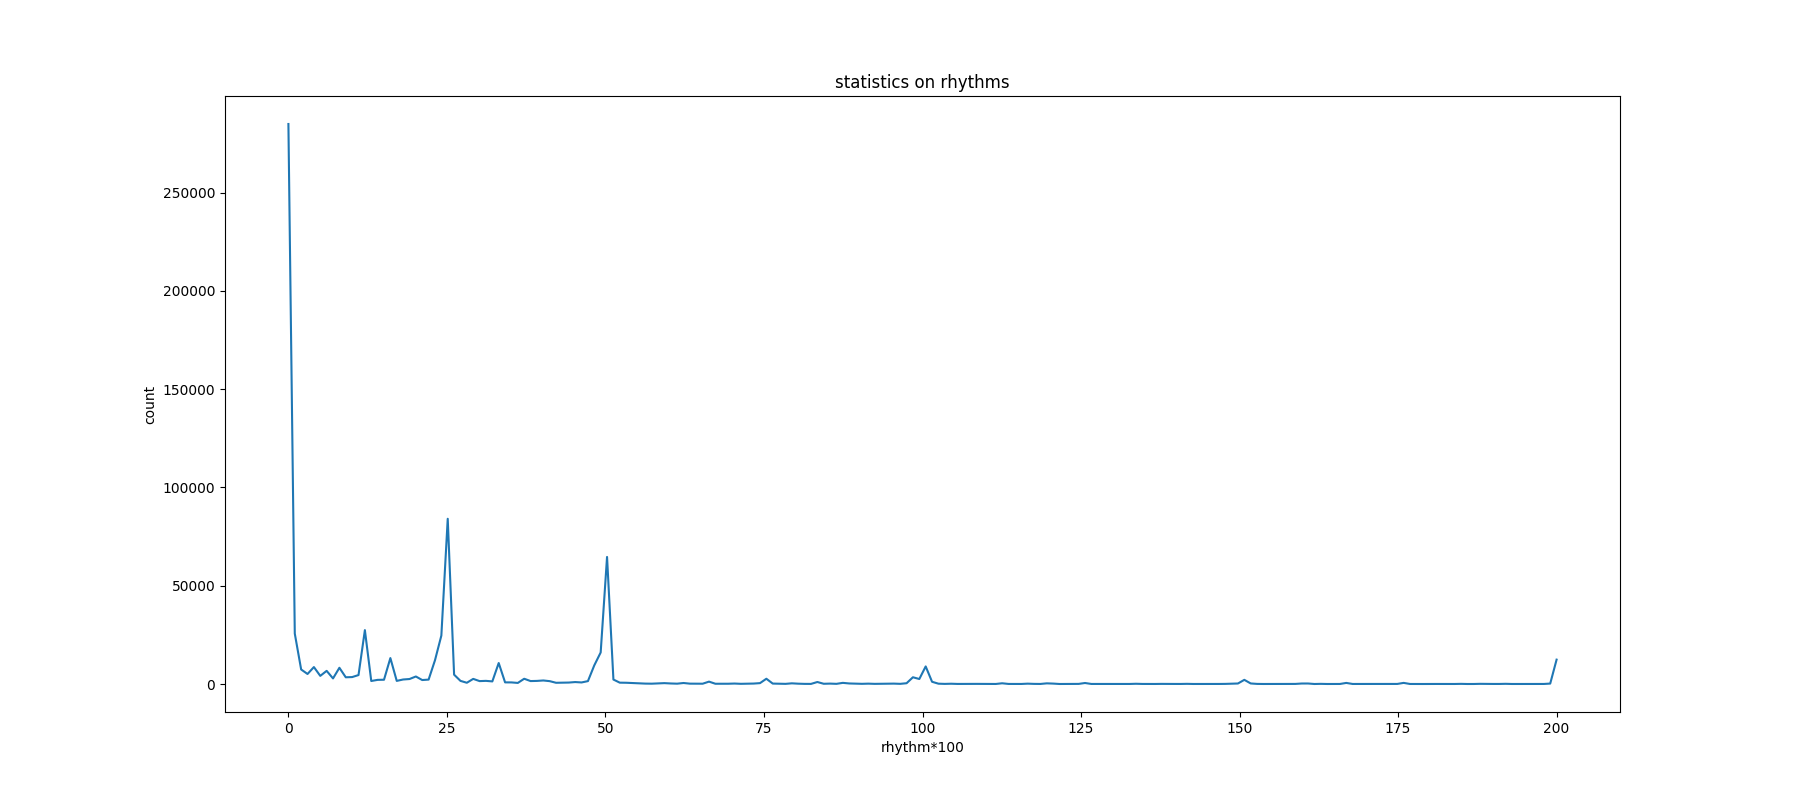
\includegraphics[width=.9\textwidth]{picture/rhythms.png}
    
    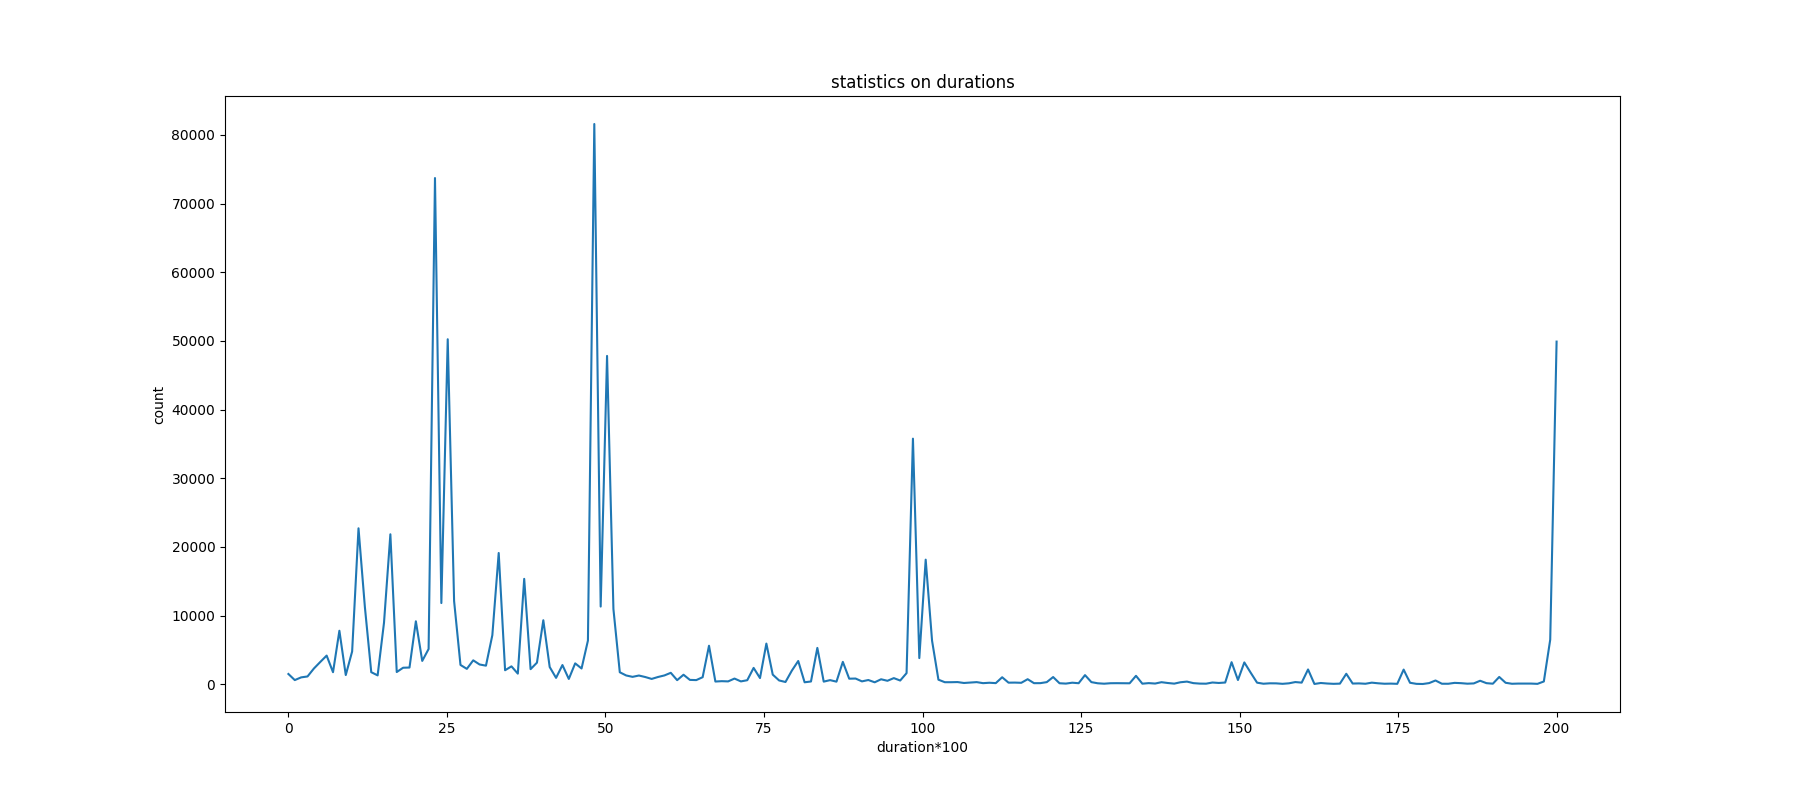
\includegraphics[width=.9\textwidth]{picture/durations.png}

    可以看出,虽然rhythmValue和duration的取值理论上是连续的,但实际上取到的值很有限,
    因此可以认为这四个要素都是离散的。基于这个事实,
    为了能够进行随机取样和关于“信息密度”的直觉判断,
    我们对输入的四个要素先分别进行one-hot编码,再连接成一个向量作为神经网络的输入。

  \subsection{结构和训练}
    我们模仿char-rnn-tensorflow构建了一个两层、每层128个神经元的递归神经网络,在输出处增加了一个隐层
    将其输出变换为和输入向量相同的长度,然后拆分为四个部分,对每部分计算softmax,
    得到音符的每个要素所有取值的概率分布,然后将其与下一个音符的one-hot编码计算交叉熵作为
    损失函数。
  \subsection{取样}
    在取样时,我们对四个要素分别进行取样。如前所述,神经网络给出了下一个音符四个要素的每种取值的概率,为了提高输出的质量,我们只考虑概率大小在平均值以上的可能取值。
  \subsection{效果}
  \label{result_of_CompoNet}
    我们做了多组实验,情况大致如下:
    \begin{itemize}
    \item 当神经网络规模为2层,每层64个神经元时,即使只使用一首曲子训练,神经网络也无法输出有规律的音符序列;
    \item 当神经网络规模为2层,每层128个神经元时,使用6首左右不太复杂的曲子,会将它们背下来;曲子数目显著增多时在可忍受的训练时间内只能输出无规律的音符序列。
    \item 如果再增大神经网络规模,还需要更多的数据来进行训练,这会显著增加对机器的要求(主要是内存大小;时间换空间很不划算)和训练所需时间,因此我们暂时做不到。
    \end{itemize}

\ifx \allfiles \undefined
\end{document}
\fi
